\chapter{Temporary}

$\max$

\section{Temporary1}
\subsection{Lemat o przedziałach zstępujących.[F38]}
Spójrzmy na fakt dotyczący granic ciągów.

\begin{theorem}[Wspólna granica dwóch ciągów monotonicznych pod porządkiem.]
Rozważmy dwa ciągi: $x_{n}$ - rosnący monotonicznie oraz $y_{n}$ - malejący monotonicznie. Ponadto załóżmy, że $x_{n}<y_{n}$ dla każdego $n\in \N$. 
Jeżeli różnica tych ciągów $y_{n}-x_{n}$ dąży do zera, to oba ciągi mają granicę skończoną:
         \[
         c = \lim x_{n}= \lim y_{n}
         .\] 
\end{theorem} 
\begin{proof}
	Istotnie, skoro dla każdego $n$ mamy $y_{n}>x_{n}$, więc w szczególności, dla każdego $n$ mamy $x_{1}< y_{n}$. Ciąg $y_{n}$ jest zatem ograniczony z dołu przez $x_{1}$, co przy jego monotoniczności pozwala wywnioskować, co pozwala wywnioskować, że jest on \textbf{zbieżny} do granicy skończonej $c = \lim_{n \to \infty} y_{n}$.

	Z analogicznego rozumowania, otrzymujemy, że ciąg $x_{n}$ jest zbieżny do granicy $c' = \lim_{n \to \infty} x_{n}$. Z arytmetyku granic wiemy, że $c-c'= \lim_{n \to \infty} \left( y_{n}-x_{n} \right)$, co po uwzględnieniu założenia, że różnica tych ciągów dąży do zera, daje nam rezultat $c=c'$. Zatem ciągi  $x_{n}, y_{n}$ zbiegają do wspólnej, skończonej granicy. 
\end{proof} 

Powyższemu twierdzeniu można nadać inną postać- w której jest częściej stosowane.
\begin{lemma}[o przedziałach zstępujących]
	Niech dany będzie ciąg przedziałów
	\[
	\langle a_1,b_1 \rangle ,\langle a_2,b_2 \rangle,\ldots\langle a_{n}, b_{n} \rangle,\ldots
	.\] 
	z których każdy następny zawiera się w poprzednim(przedziały \textbf{zstępujące}): $\langle a_{n},b_{n} \rangle \supseteq \langle a_{n+1}, b_{n+1} \rangle $, przy czym długości tych przedziałów dążą do zera wraz z wzrostem $n$ :
	\[
	\lim_{n \to \infty} (b_{n}-a_{n}) = 0
	.\] 
	Wówczas końce $a_{n}$ i $b_{n}$ (z różnych stron) dążą do wspólnej granicy \[
	c = \lim_{n \to \infty} a_{n}= \lim_{n \to \infty} b_{n}.
	.\] 
        tj. do jedynego punktu wspólnego wszystkich przedziałów(patrz obrazek).
\end{lemma} 

\begin{figure}[htpb]
	\centering
	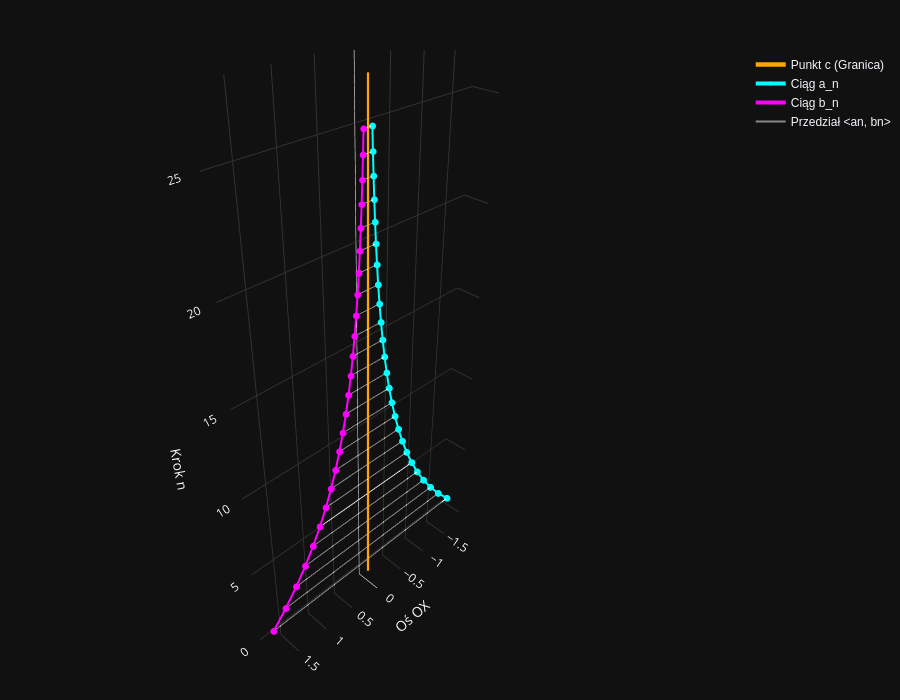
\includegraphics[width=0.8\textwidth]{nested_intervals_converging.png}
	\caption{Wizualizacja przedziałów zstępujących.}
\end{figure}


Skoro już dotknęliśmy tematykę granic, spojrzymy dokładniej na tematykę punktów skupienia oraz granicy górnej i granicy dolnej. Jakie z tego płyną analogie dla zbiorów? Zanim się za to weźmiemy, przypomnimy pewne wiadomości.
\subsection{Podciągi i punkty skupienia.[F40]} 
Niech będzie dany ciąg $\{x_{n}\} $, o wartościach $x_1,x_2,\ldots$. Rozważmy dowolny jego podciąg \[
x_{n_1}, x_{n_2}, x_{n_3},\ldots, x_{n_{k}},\ldots
.\] 
gdzie $\{n_{k}\} $ jest pewnym ciągiem rosnącym liczb naturalnych:
\[
n_1<n_2<n_3<\ldots<n_{k}<n_{k+1}<\ldots
.\] 
Tutaj rolę wskaźnika przyjmującego kolejno wszystkie wartości naturalne gra już nie n, lecz k; $\{n_{k}\} $ jest ciągiem liczb liczb naturalnych dążącym do $+\infty$ przy $k \to \infty$

\begin{fact}
	Jeśli ciąg $\{x_{n}\} $ ma określoną granicę $a$(skończoną lub nieskończoną), to tę samą granicę ma ciąg częściowy $x_{n_{k}}$
\end{fact} 
\begin{proof}
	Sprawdzimy dla przypadku skończonej liczby a. Niech dla danego $\varepsilon > 0$ istnieje takie $N$, że przy  $n>N$ jest już spełniona nierówność:  $\left| x_{n}-a \right| < \varepsilon$.

	Wobec tego, że $n_{k} \to \infty$ istnieje również takie K, że przy $k>K$ jest $n_{k} > N$. Wówczas, przy tych samych wartościach $k$ spełniona jest nierówność $\left| x_{n_{k}} - a \right| < \varepsilon$, co dowodzi naszego twierdzenia. 
\end{proof} 
\begin{remark}
	Zauważmy przy okazji, że w naszym rozumowaniu nie opieraliśmy się na monotoniczności ciągu $\{n_{k}\} $. Oznacza to, że nasze twierdzenie zachowuje moc, jeśli wskaźnik całowitoliczbowy $n_{k}$ dąży do $\infty$ według dowolnego prawa.
\end{remark} 

Jeśli ciąg $\{x_{n}\} $ nie ma określonej granicy, to nie jest wykluczone istnienie granicy dla pewnego podciągu $\{x_{n_{k}}\} $, czyli dla ciągu $x'_{k} = x_{n_{k}}$. Taką granicę nazywamy \textbf{punktem skupienia}  ciągu $\{x_{n}\} $.
\begin{eg}
	Niech $x_{n} = \left( -1 \right) ^{n+1}$, ciąg ten nie ma granicy, jeżeli jednak będziemy przebiegali tylko nieparzyste lub tylko parzyste wartości wskaźnika $n$, to podciągi
		\begin{align*}
		x_1 = 1, &x_3 = 1, \ldots, x_{2k-1} = 1, \ldots \\
		\text{oraz}\\
		x_2 = -1, &x_4 = -1, \ldots, x_{2k} = -1,\ldots
	.\end{align*}
	mają odpowiedno granic +1, -1. Liczby te są punktami skupienia ciągu $\{x_{n}\} $. Analogicznie, ciąg $x_{n} = \left( -1 \right)^{n+1}n$ ma punkty skupienia $+\infty$ i $-\infty$, a ciąg $x_{n} = n^{\left( -1 \right)^{n} + 1 }$ ma punkty skupienia $+\infty$ i $0$.

	Łatwo zbudować przykład ciągu, który ma nieskończenie wiele różnych, oto jeden z tych przykładów. Określimy ciąg $x_{n}$ następująco: jeżeli wskaźnik n ma dziesiętny zapis $b_1b_2b_3\ldots b_{j}$, to przyjmujemy $x_{n} = 0,b_1b_2b_3\ldots b_{j}$.

	Na ptzykład $x_{13} = 0.13, x_{4035} = 0.4035$ itd. \textbf{Każdy}  skończony ułamek dziesiętny pomiędzy $0.1$ a $1$ jest przyjmowany przez nasz ciąg nieskończenie wiele razy; np $0.217$ na miejscu 217, ale również 2170, 21700 itd.

	Wynika stąd od razu, że każdy skończony ułamek pomiędy $0.1$ a $1$ jest \textbf{punktem skupienia} rozważanego ciągu. Jeżeli jednak weźmiemy dowolna liczbę rzeczywistą w tym przedziale, to wystarcza ją przedstawić w postaci ułamka dziesiętnego nieskończonego:
	\[
	\alpha=0.c_1c_2\ldots c_{k}\ldots\quad (c_1\ge 1)
	.\] 
	żeby było jasne, że podciąg
	\[
	x_{c_1} = 0.c_1,\quad x_{c_1c_2}= 0.c_1c_2,\quad\ldots,\quad x_{c_1c_2\ldots c_{k}} = 0.c_1c_2\ldots c_{k},\quad \ldots
	.\] 
	dąży właśnie do $\alpha$. Tak więc w rozpatrywanym przypadku punktami skupienia ciągu są punkty przedziału $[0.1, 1]$.

	\textbf{Czy zawsze ciąg $\{x_{n}\} $ ma punkty skupienia?}

	Na to pytanie łatwo odpowiedzieć twierdząco, jeśli zbiór $\{x_{n}\} $ nie jest ograniczony. Niech np. będzie on nieograniczony z góry; wówczas dla każdego naturalnego k znajdziemy w ciągu $\{x_{n}\}$ wyraz $x_{n_{k}}$ większy niż k: $x_{n_{k}} > k \quad (k=1,2,3,\ldots)$
(przy czym łatwo dobrać wskaźniki $n_{k}$, żeby wzrastały wraz z k.) Podciąg \[
x_{n_1}, x_{n_2}, x_{n_3},\ldots,x_{n_{k}},\ldots
.\] 
ma oczywiście granicę $+\infty$. Jest to więc punkt skupienia naszego ciągu.

Również w przypadku ciągu ograniczonego można dać odpwiedź twierdzącą, ale dowód jest subtelniejszy niż w przypadku ciągu nieograniczonego.
\end{eg} 
\subsection{Lemat Bolzano-Weierstrassa.[F41]}

\begin{lemma}[Bolzano-Weierstrassa]
	Z dowolnego ciągu ograniczonego \textbf{zawsze} można wyjąć podciąg zbieżny. (To sformułowanie  nie wyklucza możliwości liczb równych w danym ciągu, co jest dogodne w zastosowaniach.)
\end{lemma}  
\begin{proof}
	Niech wszystkie liczby $x_{n}$ należą do przedziału $[a,b]$. Podzielmy ten przedział  $[a,b]$ na połowy. Wówczas choćby w jednej połowie zawarte jest nieskończenie wiele wyrazów danego ciągu, bo w przeciwnym przypadku w całym przedziale $[a,b]$ zawierałoby się tylko skończenie wiele wyrazów ciągu, co nie jest możliwe. Niech więc $[a_1,b_1]$ będzie tą połową przedziału, która zawiera nieskończenie wiele liczb $x_{n}$ (a przy obydwu połowach mających tę własność- dowolna z nich).

	Analogicznie z przedziału $[a_1,b_1]$ wydzielamy jego połowę $[a_2,b_2]$ zawierającą nieskończenie wiele liczb $x_{n}$ itd. Kontynuując to postępowanie w nieskończoność, w k-tym kroku wydzielamy przedział $[a_{k}, b_{k}]$, również zawierający nieskończenie wiele liczb  $x_{n}$.

	Każdy z utworzonych przedziałów(zaczynając od drugiego) zawiera się w poprzednim, stanowiąc jego połowę. Ponadto długość k-tego przedziału, równa 
	\[
		b_{k}-a_{k} = \frac{b-a}{2^{k}}
	.\] 
	dąży do zera wraz ze wzrostem k. Stosując \textbf{lemat o przedziałach zstępujących,} wnioskujemy, że $a_{k}$ i $b_{k}$ dążą do wspólnej granicy $c$.

	Teraz podciąg $\{x_{n_{k}}\} $ konstruujemy indukcyjnie- następująco: Jako $x_{n_1}$ dowolny, (np.pierwszy) z wyrazów $x_{n}$ naszego ciągu, zawarty w przedziale $[a_1, b_1]$. Jako $x_{n_2}$ bierzemy dowolny(np. pierwszy) z wyrazów $x_{n}$ następujących po $x_{n_1}$ i zawartych w $[a_2,b_2]$, itd. Ogólnie, jako $x_{n_{k}}$ obieramy dowolny(np. pierwszy) z wyrazów $x_{n}$, następujących po poprzednio wydzielonych wyrazach $x_{n_1}, x_{n_2}, x_{n_3},\ldots, x_{n_{k-1}}$ i zawartych w $[a_{k}, b_{k}]$. Możliwość takiego wyboru przebiegającego kolejno, zawdzięczamy temu, że każdy z przedziałów $[a_{k}, b_{k}]$ zawiera nieskończenie wiele liczb $x_{n}$, tj. zawiera elementy  $x_{n}$ o dowolnie dużych wskaźnikach.

	Dalej, ponieważ
	\[
	a_{k}\le  x_{n_{k}}\le b_{k}\text{ i } \lim a_{k}= \lim b_{k} = c,
	.\] 
	więc na mocy \textbf{twierdzenia o przedziałach zstępujących}, również $\lim x_{n_{k}} = c$ cnd.

	Metoda zastosowana przy dowodzie tego lematu, i polegająca na kolejnym dzieleniu na połowy rozważanych przedziałów, nosi nazwę \textbf{metody Bolzano}. 
\end{proof} 




\subsection{Niedokończona notatka z fichtenholza) Granice górna i dolna.[F42]}

Dowolny ciąg, czy to ograniczony, czy to nieograniczony, \textbf{ma punkty skupienia.} Udowodnimy teraz, że spośród tych punktów istnieją największy oraz najmniejszy: nazywamy je \textbf{granicą górną(łac. limes superior)} oraz \textbf{granicę dolną(łac. limes inferior)} i oznaczamy odpowiednio przez 
\[
	\limsup_{n \to \infty}  x_{n} \text{ oraz } \liminf_{n \to \infty}  x_{n}
.\] 
\begin{theorem}[Istnienie oraz równość granicy górnej i granicy dolnej.]
	Granica górna i dolna dla dowolnego ciągu $x_{n} $ \textbf{zawsze istnieją}. Ich równość jest warunkiem \textbf{koniecznym} i \textbf{dostatecznym} na istnienie granicy ciągu,
\end{theorem} 
\begin{goall} Musimy pokazać, że:
	
	\begin{enumerate}[label=\Roman*.]
		\item \textbf{Istnienie} granicy górnej i dolnej dla dowolnego ciągu $x_{n}$.
		\item \textbf{Równoważność} równości granicy górnej i dolnej z istnieniem ,,normalnej'' granicy ciągu $x_{n}$ 
	\end{enumerate}
	\end{goall} 

	Rozpatrzmy wyłączające się przypadki:
	\begin{itemize}
	\item \textbf{Ciąg $x_{n}$ nie jest ograniczony z góry:}
	
	Czyli $\forall\left(M>0\right)\exists\left(n\in N\right)\left( x_{n} >M \right).$

	Wiemy, z poprzednich ustępów(F40), że możemy wybrać(zawsze) podciąg $x_{n_{k}}$, taki że $\lim\nolimits_{k \to \infty} x_{n_{k}} = +\infty$. W tym przypadku $+\infty$ jest punktem skupienia i oczywiście największym z możliwych, a więc $\limsup_{n \to \infty} x_{n} = +\infty$.
	\item \textbf{Ciąg $x_{n}$ jest ograniczony z góry:}
	
	Czyli $\exists\left(M>0\right)\forall\left(n\in N\right)\left( x_{n} < M \right) $

	Rozważmy teraz ciąg $M_{k}$- ciąg supremum wartości ciągu $x_{n}$ począwszy od wartości $x_{k+1}$.
	\begin{align*}
		M _{1} &= \sup\{x_2,x_3,x_4,\ldots, x_{n},\ldots\}\\
		M _{2} &= \sup\{x_3,x_4,x_5,\ldots, x_{n},\ldots\}\\
		M _{3} &= \sup\{x_4,x_5,x_6\ldots, x_{n},\ldots\}\\
		           & \ldots \\
		M _{k} &= \sup\{x_{k+1}, x_{k+2},x_{k+3}\ldots\}
	.\end{align*}

	\textbf{Zauważmy,} że gdy k rośnie wartość ciągu $M_{k}$ może \textbf{tylko} maleć. Dlaczego? $M$ jest to supremum całego ciągu $x_{n}$, zatem $M_1$- supremum ,,ogonu'' ciągu  $x_{n}$($x_{n} \text{ bez }x_1$) jest \textbf{conajwyżej} tak duże jak $M$ tzn $M\ge M_1$. Analogicznie wartość $M_2$, jest \textbf{conjawyżej} tak duże jak $M_1$. Mamy tu zatem ciąg wartości zstępujących: \[
	M \ge M_1 \ge M_2 \ge M_3 \ge \ldots
	.\]  
	Ciąg $M_{k}$ jest zatem ograniczony z góry przez $M$ oraz monotonicznie malejący, zatem posiada on granicę $\lim\nolimits_{k \to \infty} M_k$, która jest albo skończona albo równa $-\infty$.
	
	Mamy zatem dwie możliwości:
	\begin{itemize}[label=$\ast$]
		\item $\bm{ \lim\nolimits_{k \to \infty} M_{k} = -\infty } $: 

			Pokazujemy, że $\lim\nolimits_{n \to \infty} x_{n} = -\infty$, czyli że $\forall\left(E'>0\right)\exists\left(N>0\right)\forall\left(n>N\right)  \left(x_{n}<-E  \right).$
	
			Zauważmy, że założenie $\lim\nolimits_{k \to \infty} M_{k} = -\infty $ mówi nam, że dla każdego $E > 0$, istnieje $k>0$, takie że $M_{k}< -E$. Weźmy zatem $N=k$, wtedy dla każdego  $n >N = k$,  $x_{n} < -E$. Z dowolnośći wyboru $E$, wnioskujemy, że $\lim\nolimits_{n \to \infty} x_{n} = -\infty$.
			Zatem istnieje granica $\lim_{n \to \infty} x_{n} = -\infty$. 
		\item $\bm{ \lim\nolimits_{k \to \infty} M_{k} = a } $ gdzie $\bm{ a } $ jest skończone:

			Pokazujemy, że $\lim\nolimits_{n \to \infty} x_{n} = a$, czyli że $\forall\left(E'\right)\exists\left(N>0\right)\forall\left(n>N\right) \left| x_{n}-a \right| < E'$.


	\end{itemize}
	
\end{itemize}

\begin{proof}
	
	 która równocześnie jest granicą górną i dolną.
	 \begin{remark}
	 	Jeżeli istnieje granica zwykła, to wszystkie punkty skupienia ciągu są jej równe
	 \end{remark} 

	 Pozostaje rozważyć najważniejszy przypadek gdy istnieje skończona granica
	 \[
	 \lim M_{k} = M^{\ast}
	 .\] 
	 Pokażemy, że liczba $M^{\ast}$ jest wówczas szukaną granicą górną ciągu $\{x_{n}\} $.

	 W tym celu ustalmy dwie własności własności charakterystyczne liczby $M^{\ast}$.

	 Jeżeli weźmiemy dowolna liczbę $\varepsilon>0$, to istnieje takie $k=N'$, że $M_{N'} < M^{\ast}+\varepsilon$ ; ponieważ przy $n>N'$ jest $x_{n}\le  M_{N'}$ to również i $x_{n}< M^{\ast}+\varepsilon$. W ten sposób otrzymaliśmy pierwszą własność. 
	 
		 \textbf{I własność liczby $M^{\ast}$:} Dla dowolnego $\varepsilon>0$ istnieje taki wskaźnik $N'$, że dla $n>N'$ jest
			 \[
			 x_{n}< M^{*}+\varepsilon
			 .\] 
	 Z drugiej strony przy dowolnym $\varepsilon>0$ i dowolnym k jest
	 \[
	 M_{k}\ge M^{*}> M^{*}-\varepsilon
	 .\] 
	 W takim razie na podstawie własności kresy górnego, spośród wartości $x_{n}$ o wskaźnikach $n=k+1, k+2,\ldots$ znajdziemy takie $x_{n'}$, że $x_{n'}> M^{*}-\varepsilon$. Zamieniając dowolnie wzięty wskaźnik k na N, otrzymujemy drugą własność.

	 	\textbf{II własność liczby $M^{*}$: } Dla dowolnego  $\varepsilon>0$ i wskaźnika N istnieje wyraz $x_{n'}, n'>N$, taki że
			\[
			x_{n'}> M^{*}-\varepsilon
			.\] 
	 Podkreślmy różnicę w sformułowaniu obu własności. W pierwszym przypadku nierówność spełniona jest dla wszystkich wyrazów  $x_{n}$. W drugim przypadku nierówność jest spełniona tylko dla pewnych $x_{n}$, wśród których są jednak wyrazy o dowolnie wielkich wskaźnikach. 

	 Opierając się na powyższych własnościach, pokażemy przede wszystkim, że liczba $M^{\ast}$ jest \textbf{punktem skupienia} ciągu $x_{n}$. W tym celu należy wybrać podciąg $x_{n_{i}}$ zbieżny do $M^{*}$.

	 Obierzmy ciąg liczb dodatnich $e_{t}\to \varepsilon$. Podstawiając $n_1=1$, przypuśćmy, że wskaźniki 
	 \[
	 n_1 = 1 < n_2 < n_3 < \ldots < n_{i-1}
	 .\]
	 są już wybrane i pokażemy jak wybrać $n_{i}$. Na mocy \textbf{własności I} dla $\varepsilon=\varepsilon_{i}$ znajdziemy odpowiedni wskaźnik $N' = N_{i}$, taki że dla wszystkich $n>N_{i}$ jest $x_{n}< M^{*}+\varepsilon_{i}$. Teraz skorzystamy z \textbf{własności II}, przyjmując jak dawniej $\varepsilon=\varepsilon_{i}$, a za N obierając większy ze wskaźników $n_{i-1}$ i $Ni$ ; temu wyborowi liczby $\varepsilon$ i $N$ odpowiada wskaźnik $n'= n_{i}$. Dla niego z jednej strony
	 $x_{n_{i}} > M^{*} - \varepsilon_{i}$,
	 z drugiej zaś przy $n_{i}> N_{i}$ jest jednocześnie
	 \[
	 x_{n_{i}} < M^{*}+ \varepsilon_{i}
	 .\] 
	 Zauważmy ponadto, że $n_{i}> n_{i-1}$.

	 Dla wyrazów $x_{n_{i}}$ utworzonego indukcyjnie ciągu mamy
	 \[
	 \left| x_{n_{i}}-M^{\ast} \right| < \varepsilon_{i} \quad \left( i=2,3,4,\ldots \right) 
	 ,\] 
	 czyi $x_{n_{i}}\to M^{\ast}$

	 Na koniec ustalmy, że żaden punkt skupienia nie może przewyższać $M^{*}$. Istotnie, dla pewnego podciągu $\{x_{n_{i}}\} $ będzie $x_{n_{i}}\to a$, czyli $a$ jest jednym z punktów skupienia. Na podstawie \textbf{własności I} dla dostatecznie dalekich wskaźników (już większych niż N') jest
	 \[
	 x_{n_{i}}< M^{*}+\varepsilon
	 .\] 

	 Przechodząc do granicy, otrzymujemy, $a\le M^{*} +\varepsilon$ i na podstawie dowolności $\varepsilon$, jest
	 \[
	 a\le M^{*}
	 .\] 

	 Tak więc $M^{*}$ jest rzeczywiście największym z punktów skupienia, tj
	 \[
	 M^{*} = \limsup x_{n} 
	 .\] 
\begin{goal}
	TODO Przeprowadzić analogiczne rozumowanie dla $\liminf$
\end{goal} 

Przejdziemy teraz do dowodu ostatniej tezy twierdzenia. 
\begin{quote}
	Jeżeli istnieje granica w zwykłym sensie $\lim x_{n}$ (skończona bądź nieskończona), to wszystkie możliwe punkty skupienia pokrywają się z tą granicą i konieczność wskazanego warunku jest oczywista.
\end{quote} 

	Załóżmy teraz, że
	\[
	\limsup = \liminf
.\] 
Jeżeli wspólną wartością tych granic jest $+\infty$ lub $-\infty$ to jak widzieliśmy, istnieje granica w zwykłym sensie i ma tę samą wartość.

Niech teraz obie granice będą skończone:
\[
M^{*} = M_{*} = a
.\] 
Wówczas, zestawiając \textbf{własność I} dla liczb $M^{*}$ i $M_{*}$ m znajdziemy dla danego $\varepsilon>0$ taki wskaźnik N, że dla $n>0$ jest \[
a-\varepsilon < x_{n}< a+\varepsilon, \text{ tzn } \left| x_{n}-a \right| < \varepsilon 
.\] 
Oznacza to, że $a$ jest granicą ciągu $\{x_{n}\} $ w zwykłym sensie, co dowodzi twierdzenia.

\begin{remark}
	Zauważmy, że za pomocą tego twierdzenia łatwo się dowodzi dostateczności warunku Bolzano-Cauchy'ego. Mianowicie (zachowując poprzednie oznaczenia) z nierówności
	\[
	x_{n'} - \varepsilon < x_{n} < x_{n'}+\varepsilon \quad \text{ (dla } n \text{ oraz } n'>N)
	.\] 
	wynika bezpośrednio, że granica gó©na i dolna ciągu $\{x_{n}\} $ są skończone i różnią się co najwyżej o $2\varepsilon$. A więc, ponieważ $\varepsilon$ jest dowolne, granice te są równe, skąd już wiadomo istnienie skończonej granicy w zwykłym sensie.
\end{remark} 
\end{proof} 


\subsection{Granice górna i dolna [F42]}

Każdy ciąg, ograniczony czy nie, posiada punkty skupienia. Udowodnimy, że wśród nich istnieją największy i najmniejszy. Nazywamy je odpowiednio \textbf{granicą górną} (\textit{limes superior}) oraz \textbf{granicą dolną} (\textit{limes inferior}):
\[
    \limsup_{n \to \infty} x_{n} \quad \text{oraz} \quad \liminf_{n \to \infty} x_{n}.
\]
\subsection{Stara notatka gemini}
\begin{theorem}[Istnienie oraz związek z granicą]
    Granica górna i dolna dla dowolnego ciągu $x_{n}$ \textbf{zawsze istnieją} (mogą być niewłaściwe).
    Warunkiem koniecznym i dostatecznym istnienia zwykłej granicy $\lim_{n \to \infty} x_n$ jest równość:
    \[ \limsup_{n \to \infty} x_{n} = \liminf_{n \to \infty} x_{n}. \]
\end{theorem}

\begin{proof}
    Rozważmy konstrukcję granicy górnej (dla dolnej rozumowanie jest analogiczne).
    
    \paragraph{Przypadek 1: Ciąg nieograniczony z góry.}
    Oznacza to, że $\forall\left(M>0\right)\exists\left(n\right) (x_{n} > M)$. Możemy zatem wybrać podciąg rozbieżny do $+\infty$. Wtedy $+\infty$ jest największym punktem skupienia, więc $\limsup x_n = +\infty$.

    \paragraph{Przypadek 2: Ciąg ograniczony z góry.}
    Niech $x_n < M$ dla każdego $n$. Zdefiniujmy ciąg $M_k$ jako kresy górne ,,ogonów'' ciągu $x_n$:
    \[
        M_k = \sup \{x_k, x_{k+1}, x_{k+2}, \ldots \}.
    \]
    Zauważmy, że zbiór, z którego bierzemy supremum, zmniejsza się wraz ze wzrostem $k$. Zatem ciąg $M_k$ jest \textbf{nierosnący}:
    \[
        M \ge M_1 \ge M_2 \ge \ldots
    \]
    Ponieważ ciąg $M_k$ jest monotoniczny, posiada granicę (skończoną lub $-\infty$). Oznaczmy ją przez $M^*$:
    \[
        \lim_{k \to \infty} M_k = M^*.
    \]
    Wykażemy, że $M^*$ jest szukaną granicą górną.
    
    \medskip
    \noindent \textbf{Analiza przypadku skończonego $M^*$.}
    Liczba $M^*$ charakteryzuje się dwiema własnościami (wynikającymi z definicji kresu i granicy):
    
    \begin{enumerate}[label=\textbf{\Roman*.}]
        \item \textbf{Ograniczenie z góry dla dalekich wyrazów.}
        Dla każdego $\varepsilon > 0$ istnieje wskaźnik $N'$, taki że dla wszystkich $n > N'$:
        \[ x_n < M^* + \varepsilon. \]
        \textit{Dowód:} Skoro $M_k \to M^*$, to dla dużych $k$, $M_k$ jest blisko $M^*$. A skoro $x_n \le M_n$, to tym bardziej $x_n$ nie przekracza $M^*$ znacznie.
        
        \item \textbf{Istnienie podciągu bliskiego $M^*$.}
        Dla każdego $\varepsilon > 0$ i każdego wskaźnika $N$ istnieje wyraz $x_{n'}$ o indeksie $n' > N$, taki że:
        \[ x_{n'} > M^* - \varepsilon. \]
        \textit{Dowód:} Ponieważ $M_k \ge M^*$, to w każdym ,,ogonie'' supremum jest co najmniej $M^*$. Musi więc istnieć element dowolnie bliski tego supremum.
    \end{enumerate}

    \noindent \textbf{Wniosek 1: $M^*$ jest punktem skupienia.}
    Konstruujemy podciąg zbieżny do $M^*$. Niech $\varepsilon_i \to 0$.
    Na mocy \textbf{własności II}, dla każdego $\varepsilon_i$ możemy dobrać wyraz $x_{n_i}$ (o indeksie większym od poprzedniego), który wpada w otoczenie:
    \[ M^* - \varepsilon_i < x_{n_i} < M^* + \varepsilon_i \quad \text{(prawa nierówność z wł. I)}. \]
    Zatem $x_{n_i} \to M^*$.

    \noindent \textbf{Wniosek 2: $M^*$ jest największym punktem skupienia.}
    Przypuśćmy, że istnieje inny punkt skupienia $a > M^*$. Wtedy istniałby podciąg zbieżny do $a$. Jednak na mocy \textbf{własności I}, od pewnego miejsca wszystkie wyrazy ciągu są mniejsze niż $M^* + \varepsilon$. Dobierając $\varepsilon$ tak małe, by $M^* + \varepsilon < a$, otrzymujemy sprzeczność.
    
    Zatem $M^*$ jest największym punktem skupienia, czyli granicą górną.
\end{proof}



Rozważmy ciąg zbiorów $A_{n}$, oraz $\limsup A_{n} = lim_k sup{A_{n}: n>k} = A$. Czym jest A w kontekście $A_{n}$? Dla kolejnych k mamy:

k=1: $\sup{A_2,A_3,\ldots,A_{n},\ldots}$
k=2: $\sup{A_3,A_4,\ldots,A_{n},\ldots}$
itd.
A jest to taki zbiór- punkt skupienia, że prawie wszystkie(wszystkie oprocz skonczonej liczby), zbiory są od niego mniejsze względem relacji zawierania?
\subsection{Porównywanie wielkości nieskończenie małych.[F60]}
Załóżmy, że w jakimś badaniu rozważamy jednocześnie kilka wielkości nieskończenie małych:
\[
	\alpha, \beta, \gamma, \delta,\ldots
,\] 

które, mówiąc ogólnie, są funkcjami tej samej zmiennej, dążącej do skończonej lub nie skończonej granicy $a$.

W wielu przypadkach interesujące jest porównanie wskazanych nieskończenie małych wielkości według charakteru dążenia do zera. Za podstawę porównania dwóch nieskoczenie małych,  $\alpha$ i $\beta$, przyjmuje się zachowanie ich ilorazu (przy jednoczesnym uwzględnieniu tego, że mianownik nie równa się zero co najmniej dla wartości $x$ dostatecznie blisko a).

W tym celu ustalimy dwa określenia:
\begin{enumerate}[label=\arabic*.]
	\item Jeżeli iloraz $\frac{\beta}{\alpha}$ (a wraz z nim $\frac{\alpha}{\beta}$ )ma granicę skończoną, różną od zera, to nieskończenie małe $\alpha$ i $\beta$ mają \textbf{ten sam rząd}.
	\item Jeżeli iloraz $\frac{\beta}{\alpha}$ jest sam nieskończenie mały (a iloraz $\frac{\alpha}{\beta}$ jest nieskończenie duży), to nieskończenie małą $\beta$ nazywamy wielkością \textbf{wyższego rzędu} niż nieskończenie mała $\alpha$ i jednocześnie nieskończenie mała $\alpha$ jest wielkością \textbf{niższego rzędu} niż nieskończenie mała $\beta$, co zapisujemy \[
	\beta = o\left( \alpha \right) 
	.\]  
\end{enumerate}

Tak więc symbol $o\left( \alpha \right) $ służy za ogólne oznaczenie nieskończenie małej wielkości wyższego rzędu niż $\alpha$, obrazowo: \[
\beta = o\left( \alpha \right) \overset{\Def}{\Longleftrightarrow} \lim \frac{\beta}{\alpha} = 0
.\] 
\subsection{Definicja pochodnej.[F92]}
Niech będzie dana funkcja $y = f\left( x \right) $ określona w przedziale $\mathcal{X}$ (działamy w $\R^{1}$. Wychodząc od pewnej wartości $x=x_0$ zmiennej niezależnej nadamy jej przyrost $\Delta x >0 $ lub $\Delta x<0$ nie wychodząc poza przedział $\mathcal{X}$, taki że nowa wartość $x_0+\Delta x$ należy do tego przedziału. Wtedy wartość $y=f\left( x_0 \right) $ funkcji zostanie zastąpiona nową wartością $y+\Delta y = f\left( x_0+\Delta x \right) $, tzn zmieni się o przyrost
\[
 \Delta y= \Delta f\left( x_0 \right) = f\left( x_0+\Delta x \right) - f\left( x_0 \right) 
.\] 
Przy tych oznaczeniach definiujemy 
\begin{definition}[Pochodna]
	Granicę, przy $\Delta x$ dążącym do 0, stosunku przyrostu funkcji $\Delta y$ do odpowiadającego mu przyrostu zmiennej niezależnej $\Delta x$ :
	\[
	\lim_{\Delta x \to 0} \frac{\Delta y}{\Delta x}= \lim_{\Delta x \to 0} \frac{f\left( x_0+\Delta x \right) - f\left( x_0 \right) }{\Delta x}
	.\] 
	\textbf{o ile granica ta istnieje}, nazywamy \textbf{pochodną funkcji $y=f\left( x \right) $} względem zmiennej niezaleźnej x, dla danej jej wartosci bądź w danym punkcie $x=x_0$. 
\end{definition} 
W ten sposób pochodna dla danej wartości $x=x_0$-jeśli istnieje- jest określoną liczbą (Póki co poprzestajemy na przypadku, gdy granica ta jest skończona por. [F100]).

Jeśli ta pochodna istnieje w \textbf{całym przedziale $\mathcal{X}$}, to jest ona funkcją $x$.

Dla oznaczenia pochodnych używa się rozmaitych symboli:
\begin{align*}
	\frac{dy}{dx}\quad &\text{ lub } \quad \frac{df\left( x_0 \right) }{dx}\quad \text{ (Leibniz)} \\
	y'\quad&\text{ lub } \quad f'\left( x_0 \right)\quad\text{ (Lagrange)}\\
		Dy \quad &\text{ lub }\quad Df\left( x_0 \right)\quad \text{(Cauchy)}
.\end{align*}

W przypadku zapisu Leibniza, póki co ten ułamek jest traktowany jako \textbf{jednolite} oznaczenie. Przy temacie różniczek zobaczymy, kiedy można go traktować jako zwykły ułamek. 

Jeśli używamy \textbf{oznaczeń funkcyjnych} (termin wyjaśniony w [F106]), czyli tych z drugiej kolumny, to litera $x_0$ w nawiasach wskazuje tę wartość zmiennej niezależnej, przy której oblicza się pochodną. W wypadkach, gdy może wynikać watpliwość, względem jakiej zmiennej obliczona jest pochodna (w porównaniu z którą ustalona jest ,,prędkość zmiany funkcji''), zmienną tę zaznacza się wskaźnikiem (tutaj wskaźnik dolny)
\[
y'_{x},f'_{x}\left( x_0 \right) , D_{x}y, D_{x}f\left( x_0 \right) 
,\] 
przy czym wskaźnik $x$ nie jest związany z tą konkretną wartością $x_0$zmiennej niezależnej dla której obliczona jest pochodna.

Można powiedzieć w pewnym sensie, że \textbf{symbole jednolite} $\frac{df}{dx}$, $f'$, $f'_{x}$, $Df$, $D_{x}f$ grają rolę symbolu funkcji dla pochodnej.
\subsection{Zestawienie wzorów na pochodne.}
Zestawimy wszystkie wyprowadzone wzory:

\begin{table}[H]
    \centering
    % Definiujemy szerokość tabeli i format kolumn
    \begin{tabular}{l l l} 
        \toprule 
        & Funkcja & Pochodna  \\
        \midrule
	    1. & $y=c$ & $y' = 0$ \\
		\addlinespace
	    2. & $y = x$ & $y' = 1$ \\
		\addlinespace
	    3.1. & $y = x^{\mu}$ & $y' = \mu x ^{\mu-1}$\\  
		\addlinespace
	    3.2. & $y = \frac{1}{x}$ & $y' = -\frac{1}{x^2}$\\
		\addlinespace
	    3.3. & $y = \sqrt{x}$ & $y' = \frac{1}{2\sqrt{x} }$\\
		\addlinespace
	    4.1. & $y = a^{x}$ & $y' = a^{x}\ln a$\\
		\addlinespace
	    4.2. & $y = e^{x}$ & $y' = e^{x}$\\
		\addlinespace
	    5.1. & $y = \log_{a}x$ & \\
		\addlinespace
	    5.2. & $y = \ln x$ & \\ 
		\addlinespace
	    6. & $y = \sin x$ & \\
		\addlinespace
	    7. & $y = \cos x$ & \\
		\addlinespace 
	    8. & $y = \tg x$ & \\
		\addlinespace
	    9. & $y = \ctg x$ & \\
		\addlinespace
	    10. & $y = \arc\sin x$& \\
		\addlinespace
	    11. & $y = \arc\cos x$ & \\
		\addlinespace
	    12. & $y = \arc\tg x$ & \\
		\addlinespace
	    13. & $y = \arc\ctg x$ & \\
		\addlinespace

        \bottomrule
    \end{tabular}
\end{table}
\subsection{Wzór na przyrost funkcji [F96]} 
Udowodnimy teraz dwa proste twierdzenia, mające dalsze zastosowania.

Niech funkcja $y = f\left( x \right) $ będzie określona przedziale $\mathcal{X}$. Wychodząc z określonej wartości $x=x_0$, z tego przedziału oznaczamy przez $\Delta x$ dowolny dodatni lub ujemny przyrost x podporządkowany jedynie temu ograniczeniu, by punkt $x_0+\Delta x$ nie wyszedł poza przedział $\mathcal{X}$. Wtedy odpowiedni przyrost funkcji będzie równy
\[
\Delta y = \Delta f\left( x_0 \right) = f\left( x_0+\Delta x \right) - f\left( x_0 \right) 
.\] 

\begin{theorem}[Lokalna liniowość]
	Jeżeli funkcja $y=f\left( x \right) $ma w punkcie pochodną skończoną $y'_{x} = f'\left( x_0 \right) $, to przyrost funkcji może być przedstawiony w postaci
	\[
	\Delta f\left( x_0 \right) = f'\left( x_0 \right) \Delta x + \alpha \cdot \Delta x
	\] 
	lub krócej:
	\[
          \Delta y = y'_{x}\Delta x + \alpha\cdot \Delta x	
	,\] 
gdzie $\alpha$ jest wielkością zależną od $\Delta x$ i dążącą wraz z $\Delta x$ do zera, tzn \[
\alpha \overset{\Def}{=} \rho\left( \Delta x \right) \text{ oraz } \lim_{\Delta x \to 0} \rho\left( \Delta x \right) = 0
.\] 
\end{theorem} 
\begin{proof}
	Na podstawie samej definicji pochodnej przy $\Delta x \to 0$ mamy
	\[
	\frac{\Delta y}{\Delta x}\to y'_{x}
	.\] 
	zakładając przeto, że
	\[
	\alpha = \frac{\Delta y}{\Delta x}-y'_{x}
	.\] 
	widzimy, że i $\alpha\to 0$. Wyznaczając stąd $\Delta y$ dojdziemy do wzoru
	\[	
          \Delta y = y'_{x}\Delta x + \alpha\cdot \Delta x	
	.\] 
\end{proof} 

Ponieważ wielkość $\alpha\Delta x (\text{przy } \Delta x \to 0)$ jest nieskończenie małą rzędu wyższego niż $\Delta x$, moża używając notacji $o$, wzory te przepisać w postaci
\[
	\Delta f\left( x_0 \right) = f'\left( x_0 \right) \Delta x + o\left(\Delta x\right) 
	\] 
	lub
	\[
          \Delta y = y'_{x}\Delta x + o\left(\Delta x\right) 
	.\]

	\begin{remark}
		Dotychczas uważaliśmy, że $\Delta x > 0$ lub $\Delta x < 0$, wielkość $\alpha$ nie była określona dla $\Delta x = 0$. Gdy mówiliśmy, że $\alpha\to 0$ przy $\Delta x \to 0$, to jak zwykle przyjmowaliśmy, że $\Delta x$ dąży do 0 w dowolny sposób, nie przybierająć jednak wartości zerowej. Załóżmy teraz, ze $\alpha = 0$, gdy $\Delta x = 0$ ; wtedy- oczywiscie powyzszy wzor pozostani w mocy i dla $\Delta x$ = 0. Procz tego zależnosć $\alpha\to 0$ przy $\Delta x \to 0$ można pojmować w szerszym sensie niż dawniej, nie wyłączajac dla $\Delta x$ możliwości dążenia do 0, przechodząc miedzy innymi przez wartości zerowe.
	\end{remark} 

	Z udowodnionych wzorów wynika bezposrednio:
	\begin{theorem}[Pochodna skonczona implikuje ciąglosc]
		Jeśli funkcja $y= f\left( x \right) $ ma w punkcie $x_0$ pochodną skończoną, to funkcja ta jest w tym punkcie ciągła.
	\end{theorem} 
	\begin{proof}
		Istotnie $\Delta x \to 0$ pociąga za sobą $\Delta y \to 0.$
	\end{proof} 
\subsection{Niezmienniczość wzoru na różniczkę [F106]}

